
\documentclass{article} % For LaTeX2e
\usepackage{iclr2026_conference,times}

% Optional math commands from https://github.com/goodfeli/dlbook_notation.
\input{math_commands.tex}

\usepackage{hyperref}
\usepackage{url}
\usepackage{graphicx}
\usepackage{booktabs}


\title{Graph-Based Methods for Multi-Agent\\ NBA Trajectory Forecasting}

\author{Rohan Gautam, Angana Mondal, Thibaut Peiffer, Nahush Kolhe \\
EE-452: Network Machine Learning\\
EPFL, Spring 2025/2026 \\
\texttt{\{firstname.lastname\}@epfl.ch}
} 

% The \author macro works with any number of authors. There are two commands
% used to separate the names and addresses of multiple authors: \And and \AND.
%
% Using \And between authors leaves it to \LaTeX{} to determine where to break
% the lines. Using \AND forces a linebreak at that point. So, if \LaTeX{}
% puts 3 of 4 authors names on the first line, and the last on the second
% line, try using \AND instead of \And before the third author name.

\newcommand{\fix}{\marginpar{FIX}}
\newcommand{\new}{\marginpar{NEW}}

\iclrfinalcopy % Show author names (school report, not an anonymous submission).
\begin{document}


\maketitle

\begin{abstract}
% 1 paragraph: task (NBA C=8 -> H=12, single-shot mean-MSE / ADE); we sweep the
% graph taxonomy but the paper centers on TWO winners -- EqMotion (exactly
% O(2)-equivariant) and augmented MART (soft O(2) invariance via augmentation);
% headline = 0.70 aug-MART + 0.30 EqMotion blend, Kaggle 2.98; central insight =
% the residual error is an irreducible ball-multimodality FLOOR (7-way confirmed).
\end{abstract}

\section{Introduction}
\label{sec:intro}
% - Problem & motivation: multi-agent human motion forecasting, NBA highlights.
% - Why it's hard: stochastic futures, agent interactions, heterogeneity
%   (players vs ball, two teams), variable-length sequences.
% - Why graphs: entities as nodes, interactions as edges, message passing.
% - Contributions (3): (i) two strong graph models + the hard-vs-soft
%   equivariance trade-off between them; (ii) court-frame (hoop) features +
%   normalization/metric-hygiene ablations; (iii) a critical 7-way analysis that
%   the error is a task floor dominated by the ball.

\section{Problem Setup \& Data}
\label{sec:setup}
% - Task: given C=8 frames predict H=12 for all N=11 entities (10 players+ball);
%   20-step windows sampled from longer sequences.
% - Data: L x N x D tensors, features [x, y, isplayer, team]; ~6K plays.
% - Protocol: local train/val fold (497 seqs) is the labelled proxy (test is
%   unlabelled); Kaggle as external reference. Metric hygiene (see 4.1).
% The metric (positions only, single-shot) is:
\begin{equation}
\label{eq:ade}
\mathrm{ADE} = \frac{1}{H\times N}\sum_{t=C+1}^{C+H}\sum_{n}
\big\lVert \hat{z}^n_t - z^n_t \big\rVert_2^2,
\qquad \hat{z}^n_t, z^n_t \in \mathbb{R}^2 .
\end{equation}

\section{Method}
\label{sec:method}

\subsection{Survey of graph paradigms (breadth)}
\label{sec:survey}
% COMPRESS to ~1 sentence each -- these are the breadth-table rows, not depth:
% temporal baseline (no graph); fixed-structure STGCNN; hypergraph GroupNet;
% dynamic/learned dNRI; multimodal STGCNN-CVAE / SocialVAE (and why single-shot
% mean-MSE penalizes best-of-K models). Establishes we covered the taxonomy.

\subsection{Equivariance: EqMotion}
\label{sec:eqmotion}
% Exactly O(2)-equivariant backbone. Our levers: isotropic normalization
% (prerequisite -- aniso norm silently breaks equivariance) + court-frame hoop
% nodes (re-inject the D2 frame as features). Key limitation: symmetry is free
% but augmentation is a no-op (reflection-TTA exact) -> it CANNOT scale capacity.

\subsection{Augmented MART}
\label{sec:augmart}
% Non-equivariant relational transformer. Soft O(2) INVARIANCE via continuous
% O(2)+mirror augmentation -> regularizes a 7.5M model over 5000 epochs with
% ZERO overfit (train~=val). Hoops transfer here too. The lever EqMotion can't use.

\subsection{The equivariance trade-off \& production blend}
\label{sec:tradeoff}
% Headline framing: an over-strong O(2) prior + explicit D2 court features beats
% BOTH plain equivariance AND learned-via-augmentation. Hard (free, can't scale)
% vs soft (paid, scales). Production = 0.70 aug-MART + 0.30 EqMotion blend.

\section{Results}
\label{sec:results}

All numbers are \texttt{val/mse\_ft}: the single-shot mean squared error in
feet$^2$ over the $H{=}12$ horizon, evaluated on the 11 real entities of the
held-out validation fold (497 sequences), matching the Kaggle ADE definition
(Eq.~\ref{eq:ade}). We report Kaggle scores where a submission was made.

\subsection{Setup \& metric hygiene}
\label{sec:hygiene}
Before comparing models we fixed two measurement artifacts, each of which moved
the apparent error by $0.2$--$0.5$~ft$^2$. \textbf{(i)~Window noise:} drawing one
random window per sequence per epoch made \texttt{val/mse\_ft} bounce between
$3.2$ and $3.9$ across epochs, so checkpoint-on-minimum selected lucky draws; a
deterministic sampler with 8 evenly-spaced windows per sequence gives a stable
selection signal. \textbf{(ii)~Landmark deflation:} when the static hoop nodes
(Sec.~\ref{sec:eqmotion}) are added, naively averaging over all 13 nodes includes
two near-zero-error stationary hoops and deflates the metric
($2.82\times13/11=3.33$); a landmark-aware metric strips them so it matches the
11-entity Kaggle score. After both fixes the validation metric tracks Kaggle
closely (e.g.\ $3.33$ val vs $3.2$ Kaggle), and the validation$\rightarrow$Kaggle
gap is consistently favorable ($\sim{+}0.08$, val is slightly pessimistic), so we
treat the local fold as a trustworthy selector.

% FIGURE 1 -- export from wandb: overlay val/mse_ft vs epoch for the noisy
% single-window run vs the deterministic --full-val run (two lines). Shows the
% selection signal stabilizing. Optional; cut first if space is tight.

\subsection{Main comparison}
\label{sec:main-results}
Table~\ref{tab:main} collects the families we explored. Two patterns stand out.
First, every graph model that predicts a single trajectory beats the non-graph
temporal baseline, while the multimodal generative models (STGCNN-CVAE,
SocialVAE) \emph{lose}: they optimise best-of-$K$ (minADE), whereas the leaderboard
scores a single-shot mean, which rewards predicting the conditional mean.
Second, our two strongest models come from opposite ends of the equivariance
spectrum (Sec.~\ref{sec:tradeoff}): the exactly-O(2)-equivariant EqMotion and the
non-equivariant augmented MART. The augmented MART backbone alone
($3.11$~val\,/\,$3.01$~Kaggle) already beats the 5-seed EqMotion ensemble, and a
$0.70$\,/\,$0.30$ blend of the two is our production submission at
\textbf{$2.98$~Kaggle}.

\begin{table}[t]
\caption{Main comparison across model families. Lower is better; \texttt{val}
is feet$^2$ on the held-out fold, \texttt{Kaggle} is the public leaderboard.
The production blend combines the two best models (Sec.~\ref{sec:tradeoff}).}
\label{tab:main}
\begin{center}
\begin{tabular}{llcc}
\toprule
\textbf{Family} & \textbf{Model} & \textbf{val} & \textbf{Kaggle} \\
\midrule
Non-graph        & Temporal baseline                 & $\sim$3.7 & -- \\
Fixed graph      & STGCNN (pos.\ graph + autoreg.)   & $\sim$3.8 & -- \\
Multimodal       & STGCNN-CVAE                       & 4.3       & -- \\
Multimodal       & SocialVAE                         & 5.0       & -- \\
Hypergraph       & MART (300 ep, fair baseline)      & 3.79      & -- \\
Equivariant      & EqMotion, single (iso + hoops)    & 3.33      & 3.2 \\
Equivariant      & EqMotion, 5-seed ensemble         & 3.25      & -- \\
Hypergraph       & aug-MART (iso + O(2) + hoops, 7.5M, 5k ep) & 3.11 & 3.01 \\
Hypergraph       & \quad + D2 test-time augmentation & 3.08      & -- \\
\midrule
\textbf{Blend}   & \textbf{0.70 aug-MART + 0.30 EqMotion} & \textbf{3.07} & \textbf{2.98} \\
\bottomrule
\end{tabular}
\end{center}
\end{table}

\subsection{Ablations on the winners}
\label{sec:ablations}
\textbf{What the symmetry buys (EqMotion).} Starting from an anisotropically
normalized baseline ($3.69$), isotropic normalization, which restores exact O(2)
equivariance, drops the error to $3.46$, and adding the two court-frame hoop
nodes drops it further to $3.33$ -- the single biggest structural lever
(Table~\ref{tab:abl}, left). Hoops are the \emph{right amount} of court
structure: adding free-throw lines, three-point apexes or corners all hurt
monotonically (e.g.\ $3.33\rightarrow3.36\rightarrow3.42$), because those points
sit on the basket axis already encoded by the hoops and merely dilute message
passing. Reflection test-time augmentation is an \emph{exact no-op} on EqMotion
(predictions identical to 4 decimals), an empirical proof of its O(2)
equivariance -- and the reason it cannot exploit augmentation to grow.

\textbf{What augmentation unlocks (MART).} A non-equivariant MART trained with the
same court inductive structure supplied as \emph{augmentation} (continuous O(2)
rotation + mirrors about court center) instead of hard equivariance can do what
EqMotion cannot: scale. Table~\ref{tab:abl} (right) shows error falling
monotonically as the schedule lengthens ($3.79\rightarrow3.55\rightarrow
3.47\rightarrow3.11$) with a 7.5M-parameter model that shows \emph{zero}
overfitting (train$\,\approx\,$val$\,\approx\,0.026$). Two diagnostics confirm
$3.11$ is a genuine model/data floor rather than a tuning artifact: budget-matched
SGDR warm restarts tie it ($3.116$), and a 10k-epoch single-cosine run does not
beat it. The remaining free gains come from variance reduction orthogonal to the
backbone: D2 test-time augmentation ($-0.03$, and its non-zero per-transform
spread \emph{measures} aug-MART's departure from exact equivariance) and the
EqMotion blend ($-0.04$).

\begin{table}[t]
\caption{Ablations on the two winning models. \textbf{Left:} EqMotion structural
levers (honest 11-entity metric). \textbf{Right:} augmented MART scaling --
augmentation is what lets the larger model and longer schedule pay off.}
\label{tab:abl}
\begin{center}
\begin{tabular}{lc@{\hspace{2.5em}}lc}
\toprule
\multicolumn{2}{c}{\textbf{EqMotion levers}} & \multicolumn{2}{c}{\textbf{aug-MART scaling}}\\
\cmidrule(r){1-2}\cmidrule(l){3-4}
Variant & val & Variant & val \\
\midrule
aniso + cosine            & 3.69 & MART 300 ep (aniso, no aug)   & 3.79 \\
\;+ isotropic norm        & 3.46 & aug iso, no hoops, 1k ep      & 3.55 \\
\;+ hoop nodes            & 3.33 & aug iso + hoops, 1k ep        & 3.47 \\
\;+ 5-seed ensemble       & 3.25 & aug iso + hoops, 5k ep        & \textbf{3.11} \\
\bottomrule
\end{tabular}
\end{center}
\end{table}

\begin{figure}[t]
\begin{center}
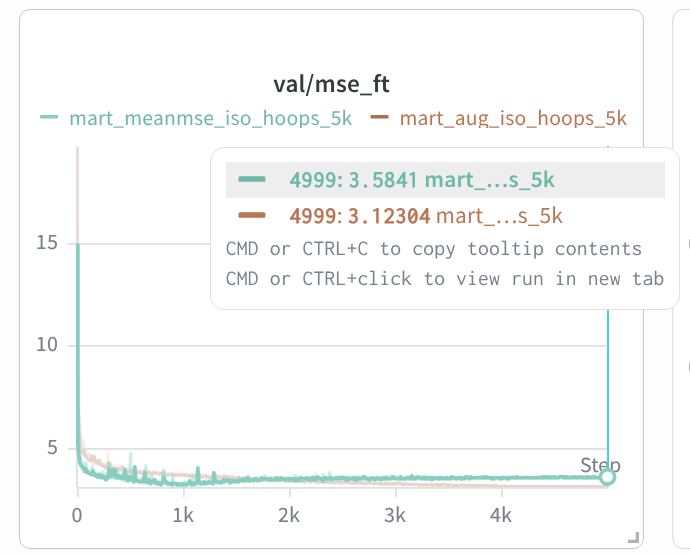
\includegraphics[width=0.62\linewidth]{fig2.png}
\end{center}
\caption{Loss choice, controlled. Two 7.5M MART models under the identical
iso\,+\,O(2)\,+\,hoops 5000-epoch recipe, differing \emph{only} in the training
loss. The min\_ade head-averaged model (orange) converges to $3.12$; direct
\texttt{mean\_mse} regression on the single-shot target (green) reaches its best
$\sim$$3.2$ early and then \emph{overfits}, ending at $3.58$. Optimising the
leaderboard metric directly is worse -- the diverse-head averaging acts as a
regularizer on the conditional mean (Sec.~\ref{sec:ball}).}
\label{fig:loss}
\end{figure}
% TODO neaten: clamp y-axis to ~[2.8, 6] so the green dip-and-rise (overfit) is
% visible; both curves are currently squished by the 0-15 range.

\subsection{The ball is the bottleneck}
\label{sec:ball}
Decomposing the error by entity reveals where the residual lives: for the
production blend the 10 players sit at $2.05$~ft$^2$ while the ball is at
$13.3$~ft$^2$ -- $6.5\times$ harder and, given the $10{:}1$ entity ratio,
essentially the \emph{entire} gap between our $3.1$ and the $2.6$ leaderboard top
(a $2.6$ total implies a ball near $7.9$ with players fixed; Table~\ref{tab:ball}).

We then asked whether this ball error is reducible, and found that it is a
\emph{task floor}, not an artifact of our models. Across two architectures with
opposite inductive biases (EqMotion ${\leftrightarrow}$ aug-MART error
correlation $\rho\!\approx\!0.94$, Fig.~\ref{fig:corr}) and seven independent
intervention strategies
-- added capacity, six aggregation/selection rules over MART's $K{=}20$ heads, a
learned per-agent head selector (re-run on the \emph{best} model, still only
$-5\%$), possession-anchoring (the ground-truth-handler oracle is $2\times$
\emph{worse} than the model), constant-velocity physics ($61.6$, the ball is
strongly non-ballistic), residual boosting, and direct \texttt{mean\_mse}
regression -- the ball MSE never leaves the $13$--$14$~ft$^2$ band. The
\texttt{mean\_mse} run is decisive (Fig.~\ref{fig:loss}): optimising the
single-shot target directly \emph{overfits} (best $3.20$ then climbing to $3.58$)
and loses to $3.11$, so the head-averaged conditional mean is already the
best-regularized estimator.
This also closes the generative lever: any point-estimate generative model
(MDN, flow-matching, diffusion) must submit the conditional mean under a
single-shot mean-MSE metric, and that target cannot beat $3.11$. The published
MoFlow/SocialVAE NBA wins are all on minADE (best-of-$K$), which our metric
structurally cannot exploit. The residual error is thus irreducible ball
multimodality -- which player receives the pass, and when -- that an 8-frame past
simply does not determine (Fig.~\ref{fig:play}); an oracle that picks the best of
MART's $K$ heads per sample reaches $0.45$~ft$^2$, but the winning mode sits in the
low-density tail and is unselectable from the context.

\begin{table}[t]
\caption{Per-entity error (feet$^2$). The ball dominates and is invariant to
model improvements; players are already at their floor.}
\label{tab:ball}
\begin{center}
\begin{tabular}{lccc}
\toprule
Model & total & ball & players \\
\midrule
EqMotion 5-seed ensemble          & 3.29 & 14.04 & 2.22 \\
aug-MART 5k (mean-of-$K$)          & 3.11 & 13.50 & 2.07 \\
\textbf{Production blend}          & \textbf{3.07} & \textbf{13.30} & \textbf{2.05} \\
\midrule
\emph{MART oracle min-of-$K$ (unattainable)} & \emph{0.64} & \emph{3.10} & \emph{0.39} \\
\bottomrule
\end{tabular}
\end{center}
\end{table}

\begin{figure}[t]
\begin{center}
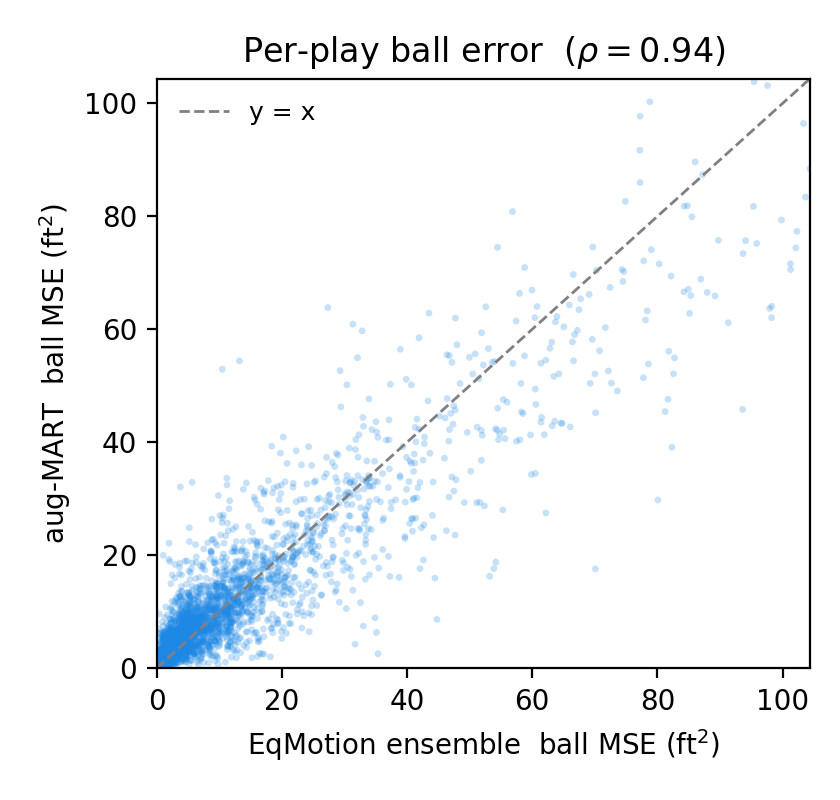
\includegraphics[width=0.40\linewidth]{fig3.png}
\end{center}
\caption{Per-play ball error, EqMotion ensemble vs.\ augmented MART, one point per
validation window. Two architectures with opposite inductive biases make the
\emph{same} errors on the \emph{same} plays ($\rho=0.94$); the residual ball error
is a property of the data, not of either model.}
\label{fig:corr}
\end{figure}

\begin{figure}[t]
\begin{center}
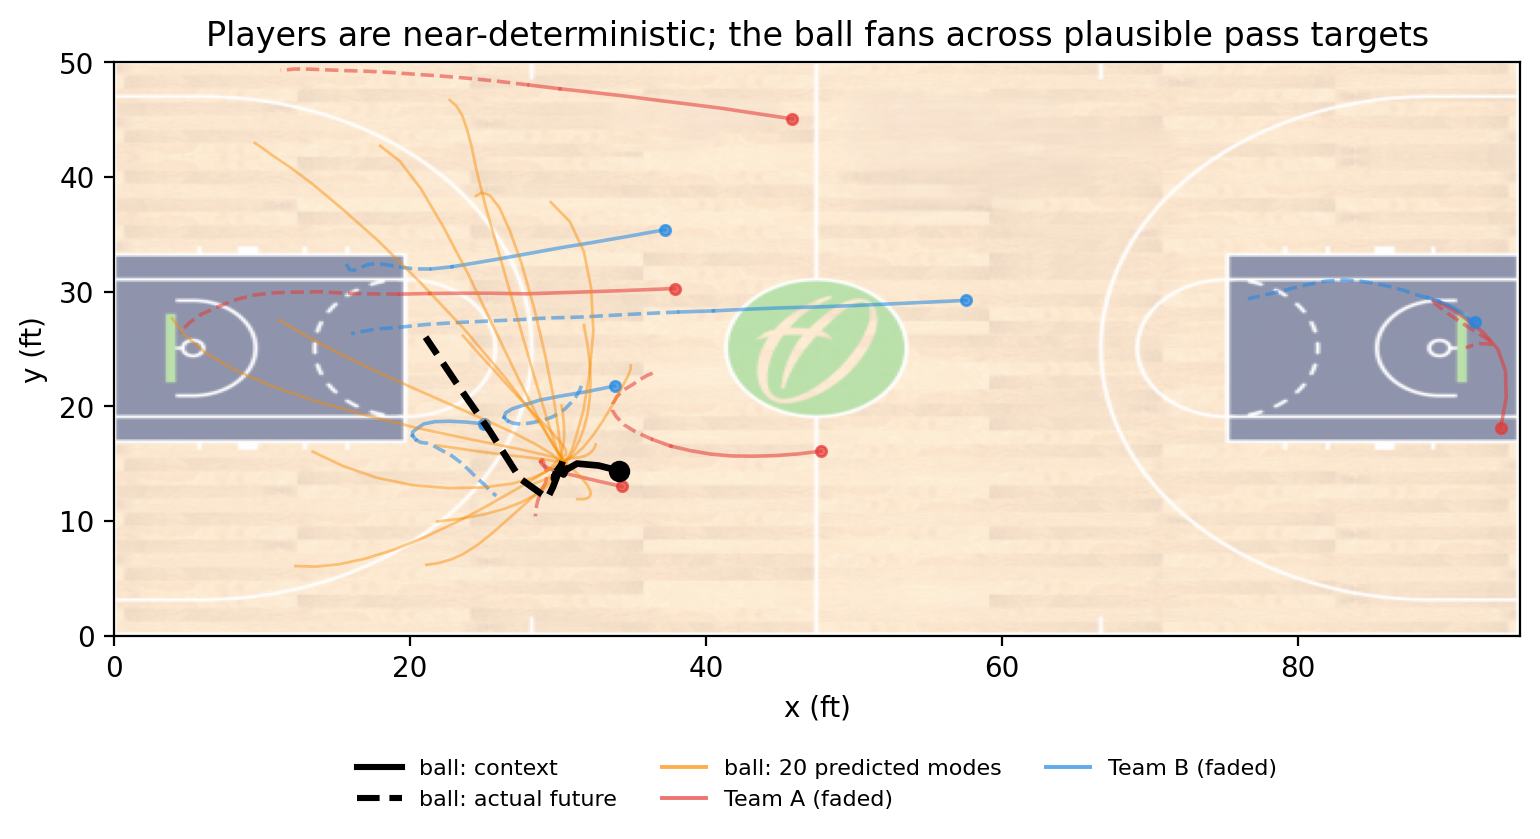
\includegraphics[width=0.92\linewidth]{fig4.png}
\end{center}
\caption{One play. Players (faded) follow near-deterministic paths the model
recovers tightly, but the ball's $K{=}20$ predicted modes (orange) fan out toward
distinct plausible pass targets, only one of which is realized (black dashed).
The mean of these modes is far from every one of them -- the source of the
irreducible ball error.}
\label{fig:play}
\end{figure}

\section{Conclusion}
\label{sec:conclusion}
% What graphs buy vs baselines; the hard-vs-soft equivariance trade-off; the
% blend (Kaggle 2.98); and the central insight -- a ball-dominated task floor.
% Limitations/future: out-of-regime info or a multi-submission mechanism (not
% available here) would be needed to pass the floor.

\appendix
\section{Appendix}
\label{sec:appendix}
% Extra tables, hyperparameters, reproducibility details.

\iffalse
% ====== ORIGINAL ICLR FORMATTING TEMPLATE (kept for reference) ======
\section{Submission of conference papers to ICLR 2026}

ICLR requires electronic submissions, processed by
\url{https://openreview.net/}. See ICLR's website for more instructions.

If your paper is ultimately accepted, the statement {\tt
  {\textbackslash}iclrfinalcopy} should be inserted to adjust the
format to the camera ready requirements.

The format for the submissions is a variant of the NeurIPS format.
Please read carefully the instructions below, and follow them
faithfully.

\subsection{Style}

Papers to be submitted to ICLR 2026 must be prepared according to the
instructions presented here.

%% Please note that we have introduced automatic line number generation
%% into the style file for \LaTeXe. This is to help reviewers
%% refer to specific lines of the paper when they make their comments. Please do
%% NOT refer to these line numbers in your paper as they will be removed from the
%% style file for the final version of accepted papers.

Authors are required to use the ICLR \LaTeX{} style files obtainable at the
ICLR website. Please make sure you use the current files and
not previous versions. Tweaking the style files may be grounds for rejection.

\subsection{Retrieval of style files}

The style files for ICLR and other conference information are available online at:
\begin{center}
   \url{http://www.iclr.cc/}
\end{center}
The file \verb+iclr2026_conference.pdf+ contains these
instructions and illustrates the
various formatting requirements your ICLR paper must satisfy.
Submissions must be made using \LaTeX{} and the style files
\verb+iclr2026_conference.sty+ and \verb+iclr2026_conference.bst+ (to be used with \LaTeX{}2e). The file
\verb+iclr2026_conference.tex+ may be used as a ``shell'' for writing your paper. All you
have to do is replace the author, title, abstract, and text of the paper with
your own.

The formatting instructions contained in these style files are summarized in
sections \ref{gen_inst}, \ref{headings}, and \ref{others} below.

\section{General formatting instructions}
\label{gen_inst}

The text must be confined within a rectangle 5.5~inches (33~picas) wide and
9~inches (54~picas) long. The left margin is 1.5~inch (9~picas).
Use 10~point type with a vertical spacing of 11~points. Times New Roman is the
preferred typeface throughout. Paragraphs are separated by 1/2~line space,
with no indentation.

Paper title is 17~point, in small caps and left-aligned.
All pages should start at 1~inch (6~picas) from the top of the page.

Authors' names are
set in boldface, and each name is placed above its corresponding
address. The lead author's name is to be listed first, and
the co-authors' names are set to follow. Authors sharing the
same address can be on the same line.

Please pay special attention to the instructions in section \ref{others}
regarding figures, tables, acknowledgments, and references.


There will be a strict upper limit of \textbf{9 pages} for the main text of the initial submission, with unlimited additional pages for citations. This limit will be expanded to \textbf{10 pages} for rebuttal/camera ready.

\section{Headings: first level}
\label{headings}

First level headings are in small caps,
flush left and in point size 12. One line space before the first level
heading and 1/2~line space after the first level heading.

\subsection{Headings: second level}

Second level headings are in small caps,
flush left and in point size 10. One line space before the second level
heading and 1/2~line space after the second level heading.

\subsubsection{Headings: third level}

Third level headings are in small caps,
flush left and in point size 10. One line space before the third level
heading and 1/2~line space after the third level heading.

\section{Citations, figures, tables, references}
\label{others}

These instructions apply to everyone, regardless of the formatter being used.

\subsection{Citations within the text}

Citations within the text should be based on the \texttt{natbib} package
and include the authors' last names and year (with the ``et~al.'' construct
for more than two authors). When the authors or the publication are
included in the sentence, the citation should not be in parenthesis using \verb|\citet{}| (as
in ``See \citet{Hinton06} for more information.''). Otherwise, the citation
should be in parenthesis using \verb|\citep{}| (as in ``Deep learning shows promise to make progress
towards AI~\citep{Bengio+chapter2007}.'').

The corresponding references are to be listed in alphabetical order of
authors, in the \textsc{References} section. As to the format of the
references themselves, any style is acceptable as long as it is used
consistently.

\subsection{Footnotes}

Indicate footnotes with a number\footnote{Sample of the first footnote} in the
text. Place the footnotes at the bottom of the page on which they appear.
Precede the footnote with a horizontal rule of 2~inches
(12~picas).\footnote{Sample of the second footnote}

\subsection{Figures}

All artwork must be neat, clean, and legible. Lines should be dark
enough for purposes of reproduction; art work should not be
hand-drawn. The figure number and caption always appear after the
figure. Place one line space before the figure caption, and one line
space after the figure. The figure caption is lower case (except for
first word and proper nouns); figures are numbered consecutively.

Make sure the figure caption does not get separated from the figure.
Leave sufficient space to avoid splitting the figure and figure caption.

You may use color figures.
However, it is best for the
figure captions and the paper body to make sense if the paper is printed
either in black/white or in color.
\begin{figure}[h]
\begin{center}
%\framebox[4.0in]{$\;$}
\fbox{\rule[-.5cm]{0cm}{4cm} \rule[-.5cm]{4cm}{0cm}}
\end{center}
\caption{Sample figure caption.}
\end{figure}

\subsection{Tables}

All tables must be centered, neat, clean and legible. Do not use hand-drawn
tables. The table number and title always appear before the table. See
Table~\ref{sample-table}.

Place one line space before the table title, one line space after the table
title, and one line space after the table. The table title must be lower case
(except for first word and proper nouns); tables are numbered consecutively.

\begin{table}[t]
\caption{Sample table title}
\label{sample-table}
\begin{center}
\begin{tabular}{ll}
\multicolumn{1}{c}{\bf PART}  &\multicolumn{1}{c}{\bf DESCRIPTION}
\\ \hline \\
Dendrite         &Input terminal \\
Axon             &Output terminal \\
Soma             &Cell body (contains cell nucleus) \\
\end{tabular}
\end{center}
\end{table}

\section{Default Notation}

In an attempt to encourage standardized notation, we have included the
notation file from the textbook, \textit{Deep Learning}
\cite{goodfellow2016deep} available at
\url{https://github.com/goodfeli/dlbook_notation/}.  Use of this style
is not required and can be disabled by commenting out
\texttt{math\_commands.tex}.


\centerline{\bf Numbers and Arrays}
\bgroup
\def\arraystretch{1.5}
\begin{tabular}{p{1in}p{3.25in}}
$\displaystyle a$ & A scalar (integer or real)\\
$\displaystyle \va$ & A vector\\
$\displaystyle \mA$ & A matrix\\
$\displaystyle \tA$ & A tensor\\
$\displaystyle \mI_n$ & Identity matrix with $n$ rows and $n$ columns\\
$\displaystyle \mI$ & Identity matrix with dimensionality implied by context\\
$\displaystyle \ve^{(i)}$ & Standard basis vector $[0,\dots,0,1,0,\dots,0]$ with a 1 at position $i$\\
$\displaystyle \text{diag}(\va)$ & A square, diagonal matrix with diagonal entries given by $\va$\\
$\displaystyle \ra$ & A scalar random variable\\
$\displaystyle \rva$ & A vector-valued random variable\\
$\displaystyle \rmA$ & A matrix-valued random variable\\
\end{tabular}
\egroup
\vspace{0.25cm}

\centerline{\bf Sets and Graphs}
\bgroup
\def\arraystretch{1.5}

\begin{tabular}{p{1.25in}p{3.25in}}
$\displaystyle \sA$ & A set\\
$\displaystyle \R$ & The set of real numbers \\
$\displaystyle \{0, 1\}$ & The set containing 0 and 1 \\
$\displaystyle \{0, 1, \dots, n \}$ & The set of all integers between $0$ and $n$\\
$\displaystyle [a, b]$ & The real interval including $a$ and $b$\\
$\displaystyle (a, b]$ & The real interval excluding $a$ but including $b$\\
$\displaystyle \sA \backslash \sB$ & Set subtraction, i.e., the set containing the elements of $\sA$ that are not in $\sB$\\
$\displaystyle \gG$ & A graph\\
$\displaystyle \parents_\gG(\ervx_i)$ & The parents of $\ervx_i$ in $\gG$
\end{tabular}
\vspace{0.25cm}


\centerline{\bf Indexing}
\bgroup
\def\arraystretch{1.5}

\begin{tabular}{p{1.25in}p{3.25in}}
$\displaystyle \eva_i$ & Element $i$ of vector $\va$, with indexing starting at 1 \\
$\displaystyle \eva_{-i}$ & All elements of vector $\va$ except for element $i$ \\
$\displaystyle \emA_{i,j}$ & Element $i, j$ of matrix $\mA$ \\
$\displaystyle \mA_{i, :}$ & Row $i$ of matrix $\mA$ \\
$\displaystyle \mA_{:, i}$ & Column $i$ of matrix $\mA$ \\
$\displaystyle \etA_{i, j, k}$ & Element $(i, j, k)$ of a 3-D tensor $\tA$\\
$\displaystyle \tA_{:, :, i}$ & 2-D slice of a 3-D tensor\\
$\displaystyle \erva_i$ & Element $i$ of the random vector $\rva$ \\
\end{tabular}
\egroup
\vspace{0.25cm}


\centerline{\bf Calculus}
\bgroup
\def\arraystretch{1.5}
\begin{tabular}{p{1.25in}p{3.25in}}
% NOTE: the [2ex] on the next line adds extra height to that row of the table.
% Without that command, the fraction on the first line is too tall and collides
% with the fraction on the second line.
$\displaystyle\frac{d y} {d x}$ & Derivative of $y$ with respect to $x$\\ [2ex]
$\displaystyle \frac{\partial y} {\partial x} $ & Partial derivative of $y$ with respect to $x$ \\
$\displaystyle \nabla_\vx y $ & Gradient of $y$ with respect to $\vx$ \\
$\displaystyle \nabla_\mX y $ & Matrix derivatives of $y$ with respect to $\mX$ \\
$\displaystyle \nabla_\tX y $ & Tensor containing derivatives of $y$ with respect to $\tX$ \\
$\displaystyle \frac{\partial f}{\partial \vx} $ & Jacobian matrix $\mJ \in \R^{m\times n}$ of $f: \R^n \rightarrow \R^m$\\
$\displaystyle \nabla_\vx^2 f(\vx)\text{ or }\mH( f)(\vx)$ & The Hessian matrix of $f$ at input point $\vx$\\
$\displaystyle \int f(\vx) d\vx $ & Definite integral over the entire domain of $\vx$ \\
$\displaystyle \int_\sS f(\vx) d\vx$ & Definite integral with respect to $\vx$ over the set $\sS$ \\
\end{tabular}
\egroup
\vspace{0.25cm}

\centerline{\bf Probability and Information Theory}
\bgroup
\def\arraystretch{1.5}
\begin{tabular}{p{1.25in}p{3.25in}}
$\displaystyle P(\ra)$ & A probability distribution over a discrete variable\\
$\displaystyle p(\ra)$ & A probability distribution over a continuous variable, or over
a variable whose type has not been specified\\
$\displaystyle \ra \sim P$ & Random variable $\ra$ has distribution $P$\\% so thing on left of \sim should always be a random variable, with name beginning with \r
$\displaystyle  \E_{\rx\sim P} [ f(x) ]\text{ or } \E f(x)$ & Expectation of $f(x)$ with respect to $P(\rx)$ \\
$\displaystyle \Var(f(x)) $ &  Variance of $f(x)$ under $P(\rx)$ \\
$\displaystyle \Cov(f(x),g(x)) $ & Covariance of $f(x)$ and $g(x)$ under $P(\rx)$\\
$\displaystyle H(\rx) $ & Shannon entropy of the random variable $\rx$\\
$\displaystyle \KL ( P \Vert Q ) $ & Kullback-Leibler divergence of P and Q \\
$\displaystyle \mathcal{N} ( \vx ; \vmu , \mSigma)$ & Gaussian distribution %
over $\vx$ with mean $\vmu$ and covariance $\mSigma$ \\
\end{tabular}
\egroup
\vspace{0.25cm}

\centerline{\bf Functions}
\bgroup
\def\arraystretch{1.5}
\begin{tabular}{p{1.25in}p{3.25in}}
$\displaystyle f: \sA \rightarrow \sB$ & The function $f$ with domain $\sA$ and range $\sB$\\
$\displaystyle f \circ g $ & Composition of the functions $f$ and $g$ \\
  $\displaystyle f(\vx ; \vtheta) $ & A function of $\vx$ parametrized by $\vtheta$.
  (Sometimes we write $f(\vx)$ and omit the argument $\vtheta$ to lighten notation) \\
$\displaystyle \log x$ & Natural logarithm of $x$ \\
$\displaystyle \sigma(x)$ & Logistic sigmoid, $\displaystyle \frac{1} {1 + \exp(-x)}$ \\
$\displaystyle \zeta(x)$ & Softplus, $\log(1 + \exp(x))$ \\
$\displaystyle || \vx ||_p $ & $\normlp$ norm of $\vx$ \\
$\displaystyle || \vx || $ & $\normltwo$ norm of $\vx$ \\
$\displaystyle x^+$ & Positive part of $x$, i.e., $\max(0,x)$\\
$\displaystyle \1_\mathrm{condition}$ & is 1 if the condition is true, 0 otherwise\\
\end{tabular}
\egroup
\vspace{0.25cm}



\section{Final instructions}
Do not change any aspects of the formatting parameters in the style files.
In particular, do not modify the width or length of the rectangle the text
should fit into, and do not change font sizes (except perhaps in the
\textsc{References} section; see below). Please note that pages should be
numbered.

\section{Preparing PostScript or PDF files}

Please prepare PostScript or PDF files with paper size ``US Letter'', and
not, for example, ``A4''. The -t
letter option on dvips will produce US Letter files.

Consider directly generating PDF files using \verb+pdflatex+
(especially if you are a MiKTeX user).
PDF figures must be substituted for EPS figures, however.

Otherwise, please generate your PostScript and PDF files with the following commands:
\begin{verbatim}
dvips mypaper.dvi -t letter -Ppdf -G0 -o mypaper.ps
ps2pdf mypaper.ps mypaper.pdf
\end{verbatim}

\subsection{Margins in LaTeX}

Most of the margin problems come from figures positioned by hand using
\verb+\special+ or other commands. We suggest using the command
\verb+\includegraphics+
from the graphicx package. Always specify the figure width as a multiple of
the line width as in the example below using .eps graphics
\begin{verbatim}
   \usepackage[dvips]{graphicx} ...
   \includegraphics[width=0.8\linewidth]{myfile.eps}
\end{verbatim}
or % Apr 2009 addition
\begin{verbatim}
   \usepackage[pdftex]{graphicx} ...
   \includegraphics[width=0.8\linewidth]{myfile.pdf}
\end{verbatim}
for .pdf graphics.
See section~4.4 in the graphics bundle documentation (\url{http://www.ctan.org/tex-archive/macros/latex/required/graphics/grfguide.ps})

A number of width problems arise when LaTeX cannot properly hyphenate a
line. Please give LaTeX hyphenation hints using the \verb+\-+ command.

\subsubsection*{Author Contributions}
If you'd like to, you may include  a section for author contributions as is done
in many journals. This is optional and at the discretion of the authors.

\subsubsection*{Acknowledgments}
Use unnumbered third level headings for the acknowledgments. All
acknowledgments, including those to funding agencies, go at the end of the paper.
% ====== END ORIGINAL TEMPLATE ======
\fi

\bibliography{iclr2026_conference}
\bibliographystyle{iclr2026_conference}

\end{document}
